%\documentclass[12pt,handout]{beamer}
\documentclass[xcolor=dvipsnames,presentation]{beamer}
\usepackage{../oop-slides-lab}
\setbeamertemplate{bibliography item}[text]

\newcommand{\lab}{Lab02}

\title[{\lab} -- Strumenti Avanzati]{Stile del Codice, Compilazione/Esecuzione avanzata di programmi Java, Programmi con Argomenti, VSCode e Debugging}

\date[\today]{\today}

\begin{document}

\frame[label=coverpage]{\titlepage}

%====================
%Outline
%====================
\begin{frame}<beamer>
    \frametitle{Outline}
    \tableofcontents[]
\end{frame}

\begin{frame}{Pre-requisiti}
\begin{itemize}
\item Rudimenti di programmazione e codifica
\item Nozioni di base dei \textbf{filesystem}
    \begin{itemize}
    \item \textbf{percorsi assoluti e relativi}
    \end{itemize}
\item Utilizzo del terminale
    \begin{itemize}
    \item interazione con il file system attraverso terminale (navigazione; concetto di working directory; etc.)
    \end{itemize}
\item \textbf{Compilazione ed esecuzione di base} di programmi Java
    \begin{itemize}
    \item uso basilare dei comandi \texttt{javac} e \texttt{java}
    \item distinzione tra file sorgenti (\texttt{.java}) e file di classi compilate (\texttt{.class})
    \item concetto di \textbf{programma/applicazione} in Java
    \end{itemize}
\item Il concetto di \textbf{package} in Java
    \begin{itemize}
    \item contenitore (organizzato gerarchicamente) di tipi (ad es. classi) che funge da namespace e permette controllo degli accessi ai tipi contenuti
    \end{itemize}
\end{itemize}
\end{frame}

\section{Stili e Convenzioni per il codice sorgente}

\begin{frame}[allowframebreaks]{Stili e Convenzioni}
    \begin{itemize}\itemsep10pt
        \item Il codice sorgente che un programmatore scrive, generalmente è \textbf{condiviso} con altre persone (del proprio team, ma anche persone esterne al team o la community)
        \begin{itemize}
            \item è importante scrivere software \textbf{immediatamente comprensibile}
            \item il fatto che un software ``giri'' (rispetti i requisiti e/o produca i risultati attesi) non è una sufficente metrica di qualità
        \end{itemize}
        \item è importante, fondamentale, adottare uno stile e seguirlo
        \begin{itemize}
            \item \textbf{chiaro} -- facilmente comprensibile
            \item \textbf{condiviso} -- piuttoto che il ``proprio stile''
            \item \textbf{consistente} --  con regole che non si contraddicono (a vari livelli)
        \end{itemize}
    \end{itemize}

\begin{block}{}
\begin{quote}
Always code as if the guy who ends up maintaining your code will be a violent psychopath who knows where you live. Code for readability.
\flushright{--- John Woods [disputed]}
\end{quote}
\end{block}

\begin{block}{Ogni linguaggio ha le sue prassi...}
\begin{itemize}
        \item Quelle Java di riferimento sono disponibili qui:
        \tiny
        \begin{itemize}
            \item \url{http://bit.ly/java-style-guide}
            \item \url{http://bit.ly/java-code-conventions}
            \item \url{http://bit.ly/oracle-java-code-conventions}
        \end{itemize}
    \end{itemize}
\end{block}

\begin{block}{Ogni azienda poi è libera di darsi altre regole interne}

\begin{itemize}
\item Ad esempio:
\footnotesize
    \begin{itemize}
        \item Google: \url{http://archive.is/a0Jhz}
         \item Twitter: \url{http://archive.is/aa1tE}
         \item Mozilla: \url{http://archive.is/rs3Ns}
    \end{itemize}
    \normalsize
\item Notare che sono sempre \textbf{consistenti}!
\begin{itemize}
\item E che sono tipicamente restrizioni delle convenzioni, non modifiche!
\end{itemize}
\end{itemize}
\end{block}

\begin{center}
\textbf{Nel corso faremo riferimento alle Java Code Conventions\\(con qualche vincolo in più)}
\end{center}
\end{frame}

\begin{frame}[allowframebreaks]{Java Code Conventions (un estratto)}
    \begin{block}{Usare \textbf{sempre} le parentesi (graffe) per if, else, for, while, anche se segue una sola istruzione}
        \begin{itemize}
            \item Aumentano la manutenibilità del codice
            \item È facile che nella fretta si modifichi il codice in modo sbagliato
            \item È facile che alcuni tool automatici si sbaglino quando ``uniscono'' pezzi di codice scritti da diverse persone
            \item Apple iOS soffrì di un grave bug a SSL/TLS causato da questa cattiva pratica \url{http://archive.is/KQp8E}
        \end{itemize}
    \end{block}
    \begin{block}{Le parentesi graffe vanno sempre ``all'egiziana'' (Egyptian brackets)}
        \begin{itemize}
            \item La graffa che apre va in linea con lo statement di apertura
            \item La graffa che chiude va in a capo, nella stessa colonna dello statement di apertura
        \end{itemize}
    \end{block}
    \begin{block}{Naming conventions - \textbf{molto importanti!}}
        \begin{itemize}
            \item I nomi di \texttt{package} usano sempre e solo lettere minuscole
            \item Usare sempre \texttt{camelCase}, evitare gli underscore (\_)
            \item I nomi di classe cominciano sempre per maiuscola: \texttt{SomeClass}
            \item I nomi di campi, metodi e variabili locali iniziano sempre per minuscola: \texttt{o.someField}, \texttt{o.someMethod()}
            \item I campi \texttt{static final} (costanti di classe) sono interamente maiuscoli e possono usare underscore
        \end{itemize}
    \end{block}

Come seguire stili e convenzioni? Tutto nelle mani del programmatore?
\begin{itemize}
\item Esistono strumenti automatici a supporto, introdotti nelle prossime lezioni...
    \end{itemize}
\end{frame}


\section{Visual Studio Code (VSCode) e Debugging}

\begin{frame}{Visual Studio Code (VSCode)}

\begin{itemize}
\item \textbf{Visual Studio Code (VSCode)} è un editor di codice sorgente leggero, versatile, e multipiattaforma
\item Estendibile attraverso un ecosistema di \textbf{estensioni} per vari linguaggi di programmazione e strumenti
	\begin{itemize}
	\item Ne vedremo alcune nei prossimi lab
	\end{itemize}
\end{itemize}

\end{frame}

\begin{frame}

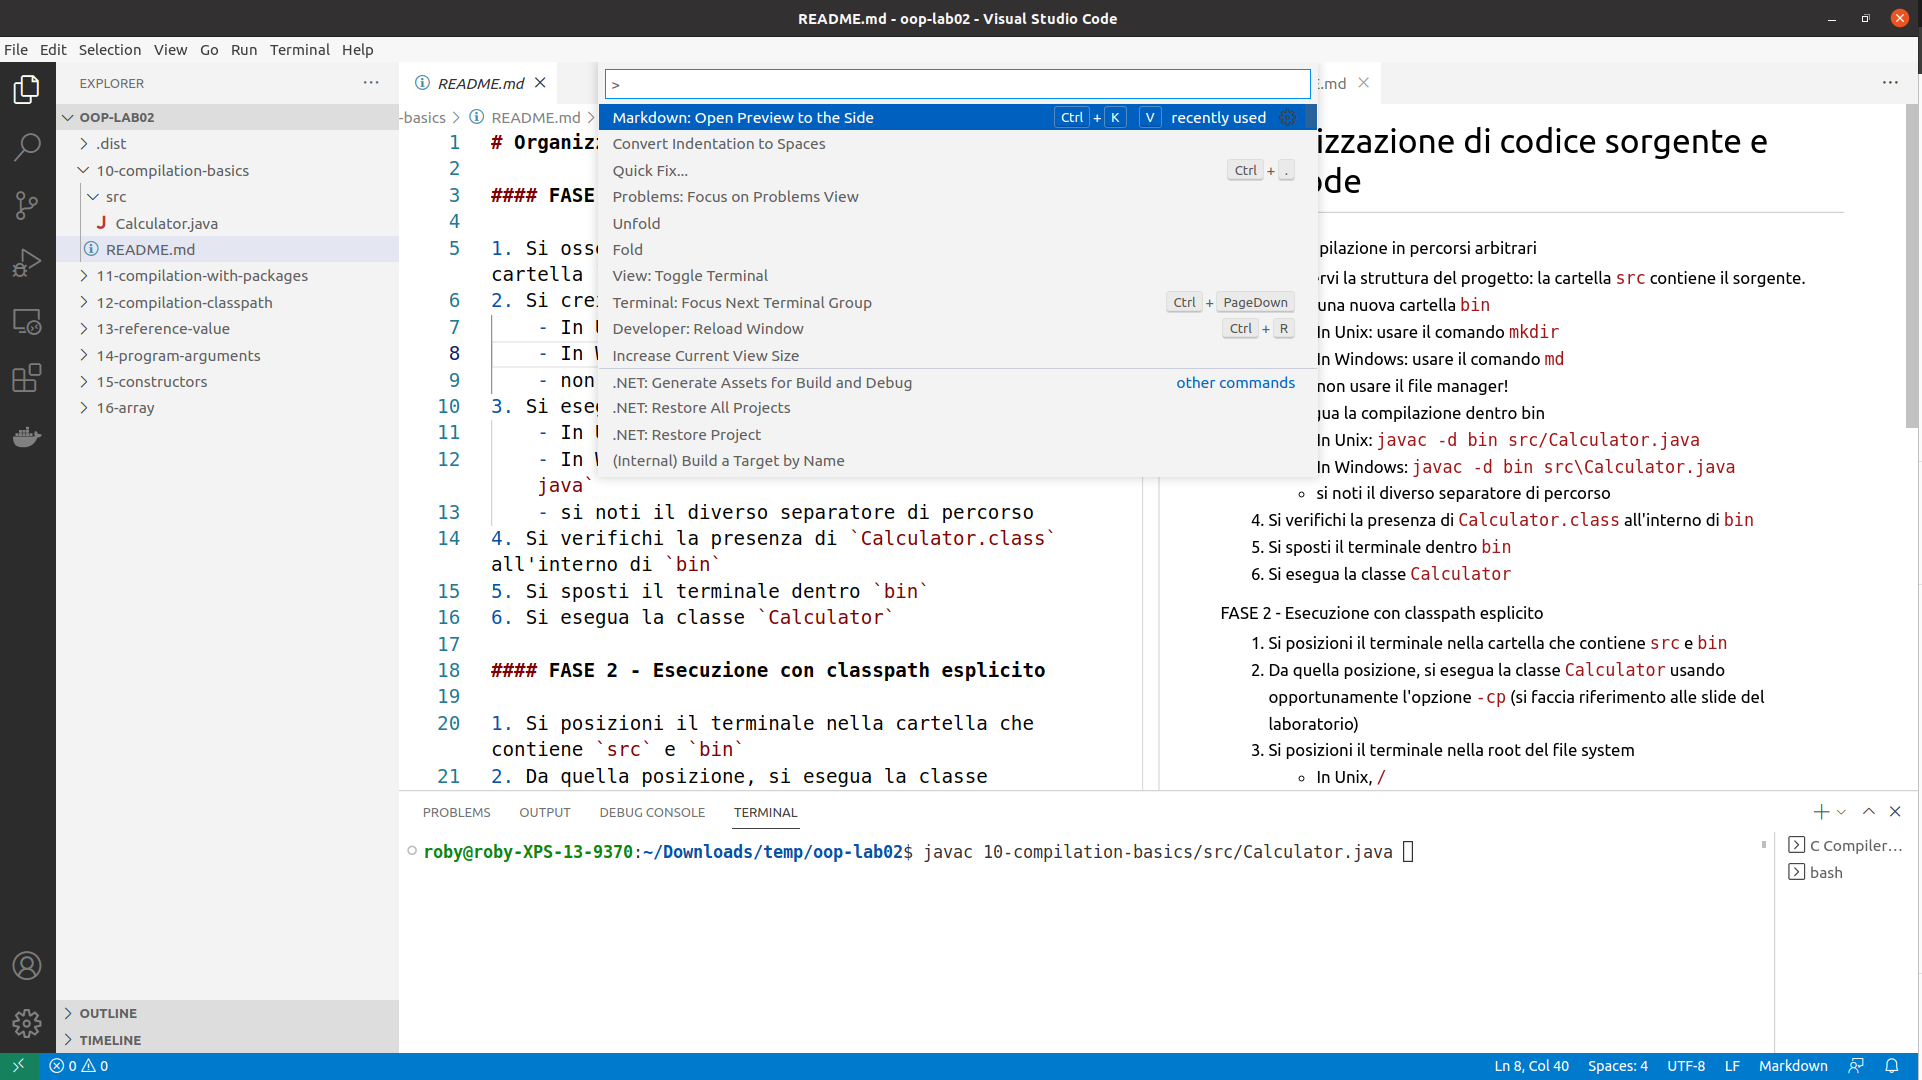
\includegraphics[width=\textwidth]{img/vscode.png}

\end{frame}

\begin{frame}{VSCode: il concetto di \textbf{workspace}}

\begin{itemize}
\item Il \textbf{workspace} è 
	\begin{enumerate}
	\item una collezione di \emph{una o più \textbf{cartelle}} aperte in una finestra (istanza di VSCode)
	\begin{itemize}
	\item Tali cartelle sono visualizzate nella vista \textbf{Explorer} sulla sinistra
	\end{itemize}
	\item più un insieme di \textbf{preferenze}, \textbf{configurazioni}, \textbf{stato}, ed \textbf{estensioni} attive memorizzate in una cartella \textbf{.vscode/}
	\end{enumerate}
\item Creazione di un workspace
	\begin{itemize}
	\item \emph{File $\to$ Open Folder}
	\end{itemize}
\item Aggiunta di cartella top-level a un workspace
	\begin{itemize}
	\item \emph{File $\to$ Add Folder to Workspace..}
	\end{itemize}
\item Salvataggio ed apertura di un workspace
	\begin{itemize}
	\item \emph{Save $\to$ Workspace as... $\to$} \emph{name}.\textbf{code-workspace} 
	\item \emph{File $\to$ Open Workspace from File}
	\end{itemize}
\end{itemize}

\end{frame}
	
\begin{frame}{Utilizzo di VSCode: alcune note}

\begin{itemize}
\item Varie scorciatoie da tastiera
	\begin{itemize}
	\item \emph{CTRL + SHIFT + P}: \textbf{command palette} (a.k.a. ``l'unico shortcut che veramente vi serve ricordare'')
	\item \emph{CTRL + SPACE}: intellisense
	\item \emph{CTRL + S}: salvataggio file corrente
	\item \emph{CTRL + PAGE UP/DOWN}: tab sorgente precedente/successivo
	\end{itemize}
\item \textbf{Apertura di un terminale:} \emph{Terminal $\to$ New Terminal}
	\begin{itemize}
	\item Sarà MOLTO UTILE
	\end{itemize}
\item \textbf{Visualizzare/installare estensioni:} \emph{File $\to$ Preferences $\to$ Extensions} oppure \emph{CTRL + SHIFT + X}
\end{itemize}

\end{frame}

\begin{frame}[allowframebreaks]{VSCode: debugging di applicazioni Java}

Nota: richiede l'estensione \textbf{Debugger for Java}

\begin{enumerate}
\item Creazione di \textbf{breakpoint} (punti di rottura del flusso di controllo)
	\begin{itemize}
	\item Click a sinistra del numero di linea di una riga di codice di interesse
	\end{itemize}
 {\centering
 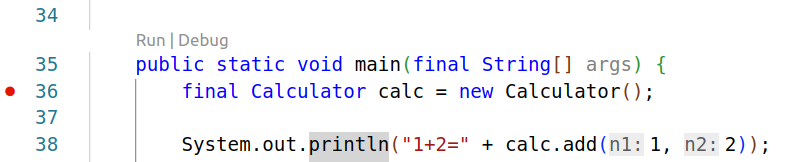
\includegraphics[height=0.15\textheight]{img/vscode-example-breakpoint2.png}
 }
\item Esecuzione di un'applicazione Java in \textbf{``modalità debug''}
	\begin{itemize}
	\item Click destro su file java $\to$ \emph{Debug Java}
	\end{itemize}
 {\centering
 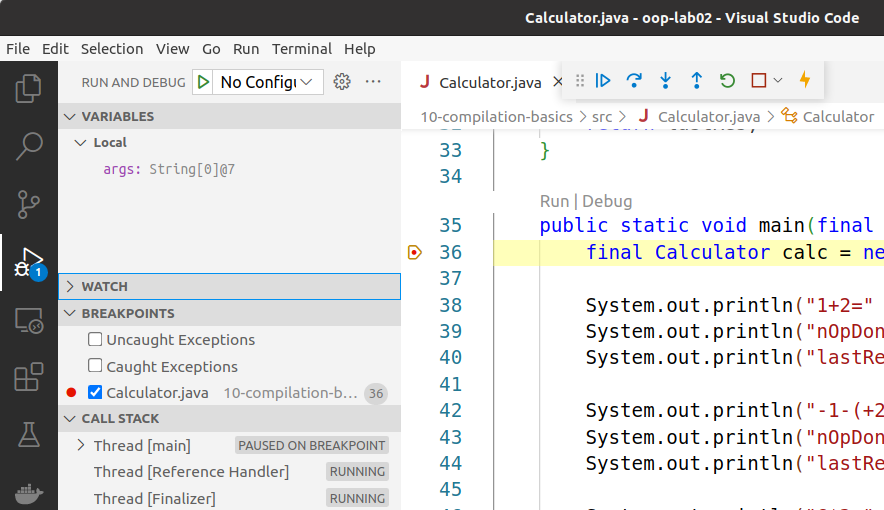
\includegraphics[height=0.4\textheight]{img/vscode-example-debug.png}
 }
\item Controllo e ispezione del comportamento runtime
	\begin{itemize}
	\item \emph{Variables}: vista che mostra le variabili in scope e il loro valore
	\item \emph{Watch}: permette di valutare espressioni rispetto al contesto d'esecuzione corrente
	\item \textbf{Step Over} (F10) o anche \emph{Run $\to$ Step Over}
	\item \textbf{Step Into} (F11)
	\item \textbf{Step Out} (SHIFT + F11)
	\item \textbf{Continue} (F5)
	\end{itemize}
\end{enumerate}

\end{frame}

\section{Compilazione ed esecuzione avanzata in Java}

\fr{Nuova opzione per \texttt{javac}}{
    \begin{itemize}
        \item Abbiamo già visto come compilare file sorgenti Java (file \texttt{.java}), generando classi in bytecode, che prendono la forma di file \texttt{.class} nella medesima directory
        \item Tuttavia è uso comune e \textbf{buona pratica} nella gestione di progetti articolati, \textbf{separare le classi sorgenti dal bytecode}, ad esempio:
    \begin{itemize}
        \item cartella \texttt{src}, per i file sorgenti (\texttt{.java})
        \item cartella \texttt{bin}, contenente le classi compilate (\texttt{.class})
    \end{itemize}
        \item Come si fa?
    \end{itemize}
    \bl{Nuova opzione del comando \texttt{javac}}{
        \iz {
            \item \cil{-d}: consente di specificare la cartella destinazione in cui compilare i file \texttt{.java}
            \item Si tratta di un'opzione che dovete obbligatoriamente saper usare
        }
        \center{\textbf{Sarà oggetto di valutazione in sede di prova pratica!}}
    }
}

\begin{frame}{Compilazione di più file da qualunque directory verso una qualunque directory}
  \begin{block}{Compilazione in directory arbitrarie}
    \texttt{javac {\color{red}-d <CARTELLA DESTINAZIONE>} <FILE JAVA>}
    \begin{itemize}
      \item \textbf{OVVIAMENTE} vanno sostituite le variabili fra parentesi angolari con le
directory che andranno usate.
    \end{itemize}
  \end{block}
  \begin{block}{Compilazione di più file in una singola passata}
    \texttt{javac -d <CARTELLA DESTINAZIONE> {\color{red}<ELENCO DI FILE JAVA>}}
    \begin{itemize}
      \item \textbf{OVVIAMENTE} vanno sostituite le variabili fra parentesi angolari con le
directory che andranno usate.
    \end{itemize}
  \end{block}
  È possibile anche utilizzare la wildcard (\texttt{*}) invece di elencare tutti i file!
  \begin{itemize}
    \item Su Unix si possono usare wildcard in più punti del path, ad esempio
\texttt{progetti/*/src/*.java} elenca tutti i file con estensione java dentro ciascuna cartella
\texttt{src} di ciascuna cartella dentro \texttt{progetti}
  \end{itemize}
\end{frame}

\begin{frame}[allowframebreaks]{Il classpath in Java}
    \begin{itemize}
        \item Il risultato della compilazione di sorgenti Java sono una o più \textbf{classi}
        	\begin{itemize}
        	\item A partire dalla cartella di destinazione (opzione \texttt{-d} di \texttt{javac}), ogni compilato \texttt{.class} sarà creato in un \textbf{sottopercorso di cartelle che corrisponde al percorso del package dichiarato per la classe corrispondente}
        	\item Ovvero, indipendentemente da dove si trovi un sorgente \texttt{C.java} definente una classe \texttt{foo.bar.C}, con \texttt{javac -d <DEST> path/to/C.java} il compilato sarà creato in \texttt{<DEST>/foo/bar/C.class}
        	\end{itemize}
        \item Quando si va ad eseguire (comando \texttt{java}), si eseguono \textbf{classi}, non files
        \begin{itemize}
            \item Infatti la virtual machine si aspetta il nome completo di una classe, il \textbf{Fully-Qualified Class Name (FQCN)}, in input
            \begin{itemize}
                \item NON il percorso al file dov'è scritta
                \item NON il percorso al file dov'è compilata
            \end{itemize}
        \end{itemize}
    \end{itemize}
    \begin{block}{Come fa la JVM a risolvere le classi?}
        \begin{itemize}
            \item Possiede un elenco di percorsi \textbf{a partire dai quali} i file compilati possono essere trovati
            \begin{itemize}
                \item All'interno di questi percorsi, i file devono essere opportunamente organizzati: \textbf{la struttura delle cartelle deve replicare quella dei package}
            \end{itemize}
            \item Cerca (in ordine) nei suddetti percorsi la classe che gli serve
            \item I percorsi possono essere directory, file compressi, o indirizzi di rete
            \item Ad esempio: se si danno i due percorsi \texttt{\color{red}/a/b/c} e \texttt{\color{blue}../foo} e si chiede di eseguire il programma definito in \texttt{{\color{black!40!green}it.unibo.}{\color{orange}Program}}, allora la JVM cercherà di caricare la classe da \texttt{{\color{red}/a/b/c/}{\color{black!40!green}it/unibo/}{\color{orange}Program}.class} o \texttt{{\color{blue}../foo/}{\color{black!40!green}it/unibo/}{\color{orange}Program}.class}
            \item Per approfondire: \url{http://archive.is/0ziau}
        \end{itemize}
    \end{block}
    \begin{center}
        L'insieme \emph{ordinato} dei percorsi prende il nome di \textbf{classpath}
    \end{center}
    \begin{block}{Default classpath}
        Se non specificato, il classpath di Java include automaticamente:
        \begin{itemize}
            \item I file jar del Java Runtime Environment
            \begin{itemize}
                \item \texttt{rt.jar} ed altri file importanti
                \item Contengono ad esempio \texttt{java.lang.Math}
            \end{itemize}
            \item La directory corrente
        \end{itemize}
    \end{block}
    \begin{block}{Aggiungere directory al classpath}
        Possono essere aggiunte directory al classpath
        \begin{itemize}
            \item Si usa l'opzione \texttt{-cp} (o, equivalentemente, \texttt{-classpath}), seguita da un elenco di percorsi
            \begin{itemize}
                \item separati dal simbolo \texttt{:} (Unix)
                \item o dal simbolo \texttt{;} (Windows)
                \item Per evitare problemi con simboli e percorsi, conviene circondare l'intero classpath con doppi apici (simbolo \texttt{"})
            \end{itemize}
        \end{itemize}
    \end{block}
\end{frame}

\begin{frame}{Più cartelle nel classpath}
    Il classpath non è composto da una sola cartella, ma può contenere più cartelle, oltre a file compressi contenenti bytecode e risorse, come zip o jar (li vedremo in futuro).
    \begin{block}{}
        Si possono specificare più cartelle utilizzando come separatore il simbolo ``\texttt{:}'' (per sistemi Unix) oppure ``\texttt{;}'' (per sistemi Windows)
        \begin{itemize}
            \item \texttt{javac -d bin -cp "lib1:lib2:lib3" src/*.java}
            \begin{itemize}
                \item Compila tutti i file con estensione java che si trovano nella cartella \texttt{src}, mettendo i compilati dentro \texttt{bin}. In compilazione, potrà linkare tutte le classi che si trovano nelle cartelle \texttt{lib1}, \texttt{lib2} e \texttt{lib3}: nel caso in cui alcuni sorgenti in src stiano usando delle classi definite dentro queste cartelle, la compilazione avrà successo.
                \item \scriptsize{Equivalente Windows: \texttt{javac -d bin -cp "lib1;lib2;lib3" src/*.java}}
        \end{itemize}
            \item \texttt{java -cp "bin:lib1:lib2:lib3" MyClass}
            \begin{itemize}
                \item Esegue il main della classe \texttt{MyClass}. Cercherà questa classe e tutte quelle collegate all'interno delle cartelle \texttt{bin}, \texttt{lib1}, \texttt{lib2} e \texttt{lib3}.
                \item \scriptsize{Equivalente Windows: \texttt{java -cp "bin;lib1;lib2;lib3" MyClass}}
            \end{itemize}
        \end{itemize}
    \end{block}
\end{frame}

\begin{frame}{Organizzazione dei sorgenti in presenza di package}
        È buona norma organizzare i sorgenti in modo da rappresentare su filesystem la struttura
dei package. Si noti però che (dato che il compilatore lavora su \alert{file}) questa scelta
\textbf{non è \underline{teoricamente} obbligatoria}!
    \begin{itemize}
        \item Lo è di fatto in questo corso, perché le cose van fatte bene
        \item Lo sarà nel mondo del lavoro, perché è prassi assolutamente comune
    \end{itemize}
    \begin{block}{Risultato della compilazione}
        Quando ad essere compilata è una classe dichiarata in un package, il compilatore
\textbf{riproduce la struttura dei package usando delle directory}
        \begin{itemize}
            \item Dato che l'interprete non lavora con file ma con \alert{classi}, il loro layout
sul file system \textbf{non può essere modificato!}
        \end{itemize}
    \end{block}
    \begin{block}{Esecuzione}
        L'esecuzione è identica al caso precedente, si faccia solo attenzione ad
usare l'intero nome della classe, che in Java include anche il nome del package!
    \end{block}
\end{frame}

\begin{frame}[fragile, allowframebreaks]{Uso del classpath in fase di compilazione}
   Supponiamo di avere in mano la seguente classe:
    \sizedcode{\tiny}{../../workspace/lab02/02-classpathcompilation/src/oop/lab02/math/UseComplex.java}
    \begin{block}{Comprensione degli errori}
        Se provassimo a compilarla da sola, potremmo ottenere degli errori
        \sizedcode{\tiny}{code/esempio3/src/oop/lab02/math/error.txt}
        \begin{itemize}
        \item Il compilatore ha bisogno di conoscere la classe \texttt{ComplexNum} per poterla
linkare e per poter compilare una classe che la riferisce
        \item Il compilatore cerca nel classpath il bytecode della classe \texttt{ComplexNum}
        \item Come risolviamo?
        \end{itemize}
    \end{block}
    \begin{block}{Utilizzo di \texttt{-cp} in fase di compilazione}
        \begin{itemize}
            \item Supponiamo di avere solo la versione compilata di \texttt{ComplexNum} (ovvero non il sorgente)
            \begin{itemize}
                \item Notate che questa è la \textit{norma} quando si usano delle librerie: vengono
                fornite già compilate!
            \end{itemize}
            \item Basterà mettere il percorso a partire dal quale \texttt{oop/lab02/math/ComplexNum.class} può essere individuata nel
            classpath di \texttt{javac}!
            \item Supponiamo di avere \texttt{UseComplex.java} nel percorso
            \texttt{src/oop/lab02/math/}
            \item Supponiamo di aver compilato \texttt{ComplexNum} con destinazione (di partenza) \texttt{lib/}
            \item Possiamo usare:
        \end{itemize}
        \alert{\texttt{javac -d bin -cp lib src/oop/lab02/math/UseComplex.java}}
    \end{block}
    \begin{block}{Spiegazione del comando}
        \texttt{javac -d bin -cp lib src/oop/lab02/math/UseComplex.java}
        \begin{itemize}
            \item \texttt{javac} $\Rightarrow$ Invocazione del compilatore
            \item \texttt{-d bin} $\Rightarrow$ \texttt{-d} determina la \textbf{destinazione}.
Vogliamo compilare dentro la cartella \texttt{bin}
            \item \texttt{-cp lib} $\Rightarrow$ \texttt{-cp} consente di aggiungere percorsi al
            \textbf{classpath}. Noi vogliamo cercare le classi che ci servono, oltre che nella
            posizione corrente e nelle librerie java, anche dentro \texttt{lib}
            \item \texttt{src/oop/lab02/math/UseComplex.java} $\Rightarrow$ Il \textit{file} che
vogliamo compilare
        \end{itemize}
    \end{block}
\end{frame}

\begin{frame}{Passare più percorsi al classpath}
    Avendo come riferimento l'esempio precedente, proviamo ad eseguire.
    \begin{itemize}
    \item Per eseguire correttamente \texttt{UseComplex} dobbiamo dire alla JVM, tramite
\textbf{-cp}, dove trovare:
    \begin{itemize}
        \item \texttt{ComplexNum}
        \item \texttt{UseComplex}
    \end{itemize}
        \item Si trovano in \textit{due percorsi diversi}!
        \item Dobbiamo specificare come argomento di \texttt{-cp} due percorsi, usando il
\textbf{separatore}:
        \begin{itemize}
            \item \textbf{\texttt{:}} su sistemi UNIX (Linux, Mac OSX, BSD)
            \item \textbf{\texttt{;}} su sistemi Windows
        \end{itemize}
        \item Useremo quindi:
        \begin{itemize}
            \item \texttt{java -cp bin:lib oop.lab02.math.UseComplex} (Unix)
            \item \texttt{java -cp bin;lib oop.lab02.math.UseComplex} (Windows)
        \end{itemize}
    \end{itemize}
\end{frame}

\begin{frame}{Esempio con sommario di funzionamento di \texttt{javac} e \texttt{java}}

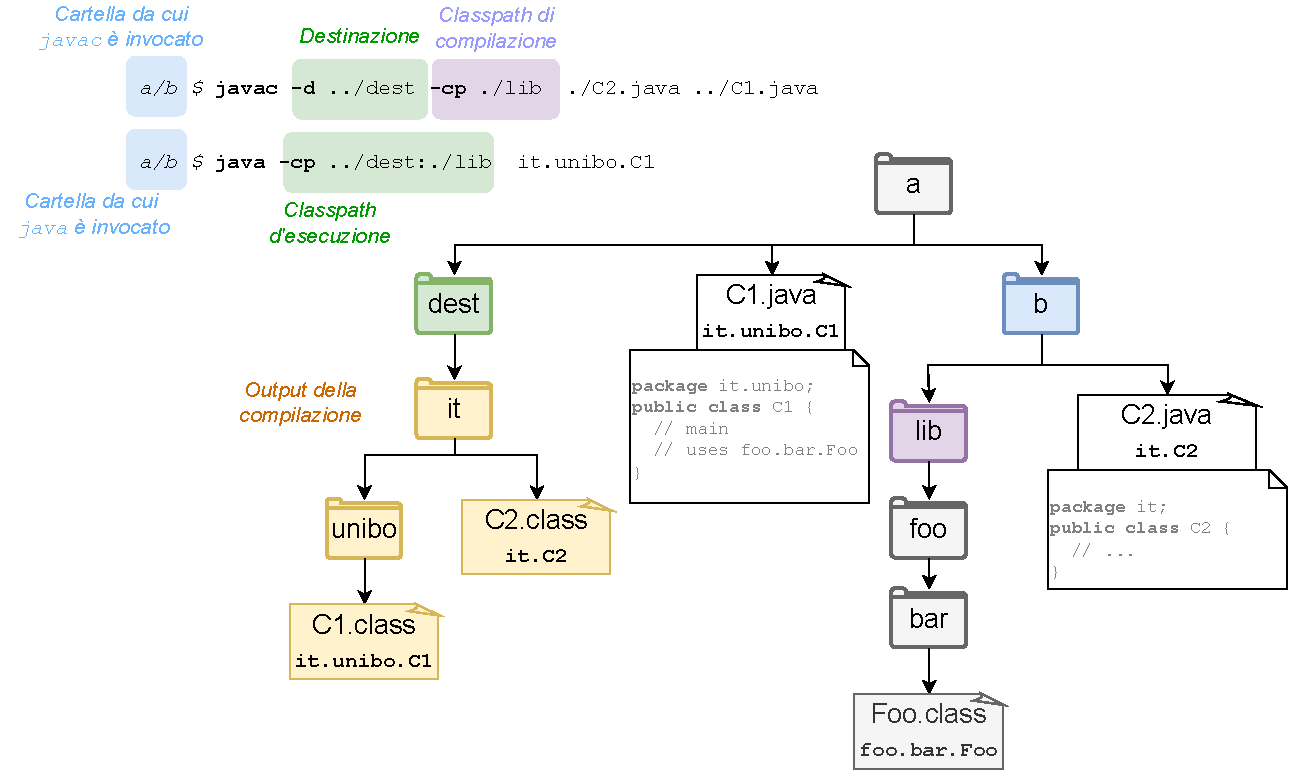
\includegraphics[width=\textwidth]{img/java-javac.drawio.pdf}

\end{frame}

\begin{frame}{Consiglio finale}
  Visto che all'esame il loro utilizzo è richiesto, è necessario imparare \textbf{a memoria} le opzioni di \texttt{java} e \texttt{javac}?
  \begin{center}
    \textbf{NO}
  \end{center}
  Entrambi i comandi (e praticamente tutti i comandi Unix) hanno con loro un'opzione che consente di stampare a video un help. Provate
  \begin{block}{}
    \begin{itemize}
      \item java -help
      \item javac -help
    \end{itemize}
  \end{block}
  \vspace{10pt}

  Gli help stampano abbondante testo con le relative istruzioni e a me serve una riga, davvero devo imparare a leggere e capire un help?
  \begin{center}
    \textbf{SÌ}
  \end{center}
  È molto facile dimenticarsi la sintassi delle opzioni di comandi che non si usano spesso. È molto più facile imparare a destreggiarsi in un help che andare a tentativi o ricordare cose a memoria.
\end{frame}

\section{Esecuzioni di programmi java con argomenti}

\begin{frame}[allowframebreaks]{Passaggio di argomenti ad un programma Java}
    \begin{itemize}\itemsep10pt
        \item La maggior parte dei comandi supporta degli argomenti
        \begin{itemize}
            \item Ad esempio, quando eseguite \texttt{javac -d bin MyClass.java} gli argomenti sono:
            \begin{enumerate}
             \item \texttt{-d}
             \item \texttt{bin}
             \item \texttt{MyClass.java}
            \end{enumerate}
        \end{itemize}
        \item In C, questi vengono passati al metodo \texttt{main()} come coppia di \texttt{char **} e \texttt{int}, rappresentanti rispettivamente un riferimento all'area di memoria dove sono salvati i parametri ed il numero dei suddetti.
        \item Anche in Java ovviamente è possibile passare degli argomenti ad un programma
        \end{itemize}

\framebreak

    \begin{itemize}\itemsep10pt
    \item La gestione è un po' più semplice che in C, grazie al fatto che gli array si portano dietro l'informazione circa la loro dimensione
        \item E grazie al fatto che la signature del metodo \texttt{main()} è una sola in Java
        \begin{itemize}
            \item \texttt{public static void main(String [])} è l'unica signature valida
            \item Mentre in C sia \texttt{int main(void)} che \texttt{int main(char **, int)} sono ugualmente accettabili
        \end{itemize}


        \item Gli argomenti con cui un programma Java viene invocato vengono passati come parametri attraverso l'array (\texttt{String[] args}) che il metodo \texttt{main()} prende in ingresso
        \begin{itemize}
        \item Nonostante sia un parametro del \emph{metodo principale} di qualunque programma Java, si tratta di un comune array senza alcuna particolarità.
        \end{itemize}

    \end{itemize}
\end{frame}

\section{Laboratorio}


\fr{Preparazione ambiente di lavoro}{
\begin{itemize}\itemsep10pt
\item Accedere al PC di laboratorio con le proprie credenziali istituzionali
        \item Accedere al sito del corso
%    \iz{
%        \item \textcolor{blue}{\url{http://bit.ly/oop19-cesena}}
%    }
    \item Scaricare il materiale dell'esercitazione odierna
    \item Spostare il file scaricato sul Desktop
    \item Decomprimere il file e aprire con Visual Studio Code la directory ottenuta (File $\to$ Open Folder...)
    \item Puntare il terminale alla directory con i sorgenti dell'esercitazione odierna
\end{itemize}
}


\subsection{Appendice: richiami utili per gli esercizi del {\lab}}

\begin{frame}{A1 -- Varianza}

\begin{block}{Formula per il calcolo della varianza}
Sia $n$ il numero di elementi dell'array ed $x_i$ l'elemento all'indice $i$ dell'array, e $\mu$ la media dei valori del suddetto array. La varianza $\sigma^2$ può essere calcolata come:

\centering
\huge
$\sigma^2 = \frac{\displaystyle\sum_{i=0}^{n-1}(x_i - \mu)^2} {n}$
\end{block}
\end{frame}

%\begin{frame}[allowframebreaks]
% \frametitle{Bibliography}
%    \bibliographystyle{plain}
%    \small
% \bibliography{biblio}
%\end{frame}


\end{document}
